\documentclass[]{article}
\usepackage{lmodern}
\usepackage{amssymb,amsmath}
\usepackage{ifxetex,ifluatex}
\usepackage{fixltx2e} % provides \textsubscript
\ifnum 0\ifxetex 1\fi\ifluatex 1\fi=0 % if pdftex
  \usepackage[T1]{fontenc}
  \usepackage[utf8]{inputenc}
\else % if luatex or xelatex
  \ifxetex
    \usepackage{mathspec}
  \else
    \usepackage{fontspec}
  \fi
  \defaultfontfeatures{Ligatures=TeX,Scale=MatchLowercase}
\fi
% use upquote if available, for straight quotes in verbatim environments
\IfFileExists{upquote.sty}{\usepackage{upquote}}{}
% use microtype if available
\IfFileExists{microtype.sty}{%
\usepackage{microtype}
\UseMicrotypeSet[protrusion]{basicmath} % disable protrusion for tt fonts
}{}
\usepackage[margin=1in]{geometry}
\usepackage{hyperref}
\hypersetup{unicode=true,
            pdftitle={Assignment4},
            pdfauthor={Syed Muhammad Adeel Ibrahim},
            pdfborder={0 0 0},
            breaklinks=true}
\urlstyle{same}  % don't use monospace font for urls
\usepackage{color}
\usepackage{fancyvrb}
\newcommand{\VerbBar}{|}
\newcommand{\VERB}{\Verb[commandchars=\\\{\}]}
\DefineVerbatimEnvironment{Highlighting}{Verbatim}{commandchars=\\\{\}}
% Add ',fontsize=\small' for more characters per line
\usepackage{framed}
\definecolor{shadecolor}{RGB}{248,248,248}
\newenvironment{Shaded}{\begin{snugshade}}{\end{snugshade}}
\newcommand{\KeywordTok}[1]{\textcolor[rgb]{0.13,0.29,0.53}{\textbf{#1}}}
\newcommand{\DataTypeTok}[1]{\textcolor[rgb]{0.13,0.29,0.53}{#1}}
\newcommand{\DecValTok}[1]{\textcolor[rgb]{0.00,0.00,0.81}{#1}}
\newcommand{\BaseNTok}[1]{\textcolor[rgb]{0.00,0.00,0.81}{#1}}
\newcommand{\FloatTok}[1]{\textcolor[rgb]{0.00,0.00,0.81}{#1}}
\newcommand{\ConstantTok}[1]{\textcolor[rgb]{0.00,0.00,0.00}{#1}}
\newcommand{\CharTok}[1]{\textcolor[rgb]{0.31,0.60,0.02}{#1}}
\newcommand{\SpecialCharTok}[1]{\textcolor[rgb]{0.00,0.00,0.00}{#1}}
\newcommand{\StringTok}[1]{\textcolor[rgb]{0.31,0.60,0.02}{#1}}
\newcommand{\VerbatimStringTok}[1]{\textcolor[rgb]{0.31,0.60,0.02}{#1}}
\newcommand{\SpecialStringTok}[1]{\textcolor[rgb]{0.31,0.60,0.02}{#1}}
\newcommand{\ImportTok}[1]{#1}
\newcommand{\CommentTok}[1]{\textcolor[rgb]{0.56,0.35,0.01}{\textit{#1}}}
\newcommand{\DocumentationTok}[1]{\textcolor[rgb]{0.56,0.35,0.01}{\textbf{\textit{#1}}}}
\newcommand{\AnnotationTok}[1]{\textcolor[rgb]{0.56,0.35,0.01}{\textbf{\textit{#1}}}}
\newcommand{\CommentVarTok}[1]{\textcolor[rgb]{0.56,0.35,0.01}{\textbf{\textit{#1}}}}
\newcommand{\OtherTok}[1]{\textcolor[rgb]{0.56,0.35,0.01}{#1}}
\newcommand{\FunctionTok}[1]{\textcolor[rgb]{0.00,0.00,0.00}{#1}}
\newcommand{\VariableTok}[1]{\textcolor[rgb]{0.00,0.00,0.00}{#1}}
\newcommand{\ControlFlowTok}[1]{\textcolor[rgb]{0.13,0.29,0.53}{\textbf{#1}}}
\newcommand{\OperatorTok}[1]{\textcolor[rgb]{0.81,0.36,0.00}{\textbf{#1}}}
\newcommand{\BuiltInTok}[1]{#1}
\newcommand{\ExtensionTok}[1]{#1}
\newcommand{\PreprocessorTok}[1]{\textcolor[rgb]{0.56,0.35,0.01}{\textit{#1}}}
\newcommand{\AttributeTok}[1]{\textcolor[rgb]{0.77,0.63,0.00}{#1}}
\newcommand{\RegionMarkerTok}[1]{#1}
\newcommand{\InformationTok}[1]{\textcolor[rgb]{0.56,0.35,0.01}{\textbf{\textit{#1}}}}
\newcommand{\WarningTok}[1]{\textcolor[rgb]{0.56,0.35,0.01}{\textbf{\textit{#1}}}}
\newcommand{\AlertTok}[1]{\textcolor[rgb]{0.94,0.16,0.16}{#1}}
\newcommand{\ErrorTok}[1]{\textcolor[rgb]{0.64,0.00,0.00}{\textbf{#1}}}
\newcommand{\NormalTok}[1]{#1}
\usepackage{graphicx,grffile}
\makeatletter
\def\maxwidth{\ifdim\Gin@nat@width>\linewidth\linewidth\else\Gin@nat@width\fi}
\def\maxheight{\ifdim\Gin@nat@height>\textheight\textheight\else\Gin@nat@height\fi}
\makeatother
% Scale images if necessary, so that they will not overflow the page
% margins by default, and it is still possible to overwrite the defaults
% using explicit options in \includegraphics[width, height, ...]{}
\setkeys{Gin}{width=\maxwidth,height=\maxheight,keepaspectratio}
\IfFileExists{parskip.sty}{%
\usepackage{parskip}
}{% else
\setlength{\parindent}{0pt}
\setlength{\parskip}{6pt plus 2pt minus 1pt}
}
\setlength{\emergencystretch}{3em}  % prevent overfull lines
\providecommand{\tightlist}{%
  \setlength{\itemsep}{0pt}\setlength{\parskip}{0pt}}
\setcounter{secnumdepth}{0}
% Redefines (sub)paragraphs to behave more like sections
\ifx\paragraph\undefined\else
\let\oldparagraph\paragraph
\renewcommand{\paragraph}[1]{\oldparagraph{#1}\mbox{}}
\fi
\ifx\subparagraph\undefined\else
\let\oldsubparagraph\subparagraph
\renewcommand{\subparagraph}[1]{\oldsubparagraph{#1}\mbox{}}
\fi

%%% Use protect on footnotes to avoid problems with footnotes in titles
\let\rmarkdownfootnote\footnote%
\def\footnote{\protect\rmarkdownfootnote}

%%% Change title format to be more compact
\usepackage{titling}

% Create subtitle command for use in maketitle
\providecommand{\subtitle}[1]{
  \posttitle{
    \begin{center}\large#1\end{center}
    }
}

\setlength{\droptitle}{-2em}

  \title{Assignment4}
    \pretitle{\vspace{\droptitle}\centering\huge}
  \posttitle{\par}
    \author{Syed Muhammad Adeel Ibrahim}
    \preauthor{\centering\large\emph}
  \postauthor{\par}
      \predate{\centering\large\emph}
  \postdate{\par}
    \date{June 1, 2019}


\begin{document}
\maketitle

\subsection{\texorpdfstring{Question 1. This question uses R S3 OOP to
manipulate regular polygons whose vertices are (by default) on the unit
circle of the plane, i.e., centred always at the origin. Write some code
to implement the following. You'll need to define a class called
``regpolygon3'' that contains information on its radius and angle
because later we allow them to change. To keep things uniform, by
default, one of the vertices is located at (0, 1). See Figure
1.}{Question 1. This question uses R S3 OOP to manipulate regular polygons whose vertices are (by default) on the unit circle of the plane, i.e., centred always at the origin. Write some code to implement the following. You'll need to define a class called regpolygon3 that contains information on its radius and angle because later we allow them to change. To keep things uniform, by default, one of the vertices is located at (0, 1). See Figure 1.}}\label{question-1.-this-question-uses-r-s3-oop-to-manipulate-regular-polygons-whose-vertices-are-by-default-on-the-unit-circle-of-the-plane-i.e.-centred-always-at-the-origin.-write-some-code-to-implement-the-following.-youll-need-to-define-a-class-called-regpolygon3-that-contains-information-on-its-radius-and-angle-because-later-we-allow-them-to-change.-to-keep-things-uniform-by-default-one-of-the-vertices-is-located-at-0-1.-see-figure-1.}

\subsubsection{\texorpdfstring{(a) Write a constructor function to
create a regular polygon with any number of sides, from 3 and upwards.
Allow for circles. Hence each object should contain the following
information: the number of sides, the coordinates of one of its
vertices, and an optional name such as ``triangle'', ``square'',
``pentagon'', ``hexagon'',. . . , ``circle''.Build in some error
checking too. For example, the number of sides should be integervalued,
the radius should be positive and finite, etc. Of course, missing values
are not allowed. Run your code to create something like the following.
{[}5
marks{]}}{(a) Write a constructor function to create a regular polygon with any number of sides, from 3 and upwards. Allow for circles. Hence each object should contain the following information: the number of sides, the coordinates of one of its vertices, and an optional name such as triangle, square, pentagon, hexagon,. . . , circle.Build in some error checking too. For example, the number of sides should be integervalued, the radius should be positive and finite, etc. Of course, missing values are not allowed. Run your code to create something like the following. {[}5 marks{]}}}\label{a-write-a-constructor-function-to-create-a-regular-polygon-with-any-number-of-sides-from-3-and-upwards.-allow-for-circles.-hence-each-object-should-contain-the-following-information-the-number-of-sides-the-coordinates-of-one-of-its-vertices-and-an-optional-name-such-as-triangle-square-pentagon-hexagon.-.-.-circle.build-in-some-error-checking-too.-for-example-the-number-of-sides-should-be-integervalued-the-radius-should-be-positive-and-finite-etc.-of-course-missing-values-are-not-allowed.-run-your-code-to-create-something-like-the-following.-5-marks}

\begin{Shaded}
\begin{Highlighting}[]
\NormalTok{newregpolygon3 <-}\StringTok{ }\ControlFlowTok{function}\NormalTok{(}\DataTypeTok{sides =} \DecValTok{3}\NormalTok{) \{}
  \ControlFlowTok{if}\NormalTok{ (sides }\OperatorTok{<}\StringTok{ }\DecValTok{2}\NormalTok{) \{}
    \KeywordTok{stop}\NormalTok{(}\StringTok{"sides should be greater than or equal to 3"}\NormalTok{)}
\NormalTok{  \} }\ControlFlowTok{else} \ControlFlowTok{if}\NormalTok{ (}\KeywordTok{is.infinite}\NormalTok{(sides)) \{}
\NormalTok{    sides <-}\StringTok{ }\DecValTok{99}
\NormalTok{  \} }\ControlFlowTok{else} \ControlFlowTok{if}\NormalTok{ (sides}\OperatorTok\DecValTok{1} \OperatorTok{!=}\StringTok{ }\DecValTok{0}\NormalTok{) \{}
    \KeywordTok{stop}\NormalTok{(}\StringTok{"sides should be integer"}\NormalTok{)}
\NormalTok{  \}}
  
  \CommentTok{# sides + 1 in order to have a closing point}
\NormalTok{  radius <-}\StringTok{ }\DecValTok{1}
\NormalTok{  shift <-}\StringTok{ }\DecValTok{0}
  
  \KeywordTok{regpolygon3}\NormalTok{(sides, radius, shift)}
\NormalTok{\}}

\NormalTok{regpolygon3 <-}\StringTok{ }\ControlFlowTok{function}\NormalTok{(sides, radius, shift) \{}
  
\NormalTok{  theta0 <-}\StringTok{ }\NormalTok{shift }\OperatorTok{+}\StringTok{ }\KeywordTok{seq}\NormalTok{(}\DecValTok{0}\NormalTok{, }\DecValTok{2} \OperatorTok{*}\StringTok{ }\NormalTok{pi, }\DataTypeTok{length =}\NormalTok{ sides }\OperatorTok{+}\StringTok{ }\DecValTok{1}\NormalTok{)}
\NormalTok{  x <-}\StringTok{ }\NormalTok{radius }\OperatorTok{*}\StringTok{ }\KeywordTok{round}\NormalTok{(}\KeywordTok{sin}\NormalTok{(theta0), }\DecValTok{4}\NormalTok{)}
\NormalTok{  y <-}\StringTok{ }\NormalTok{radius }\OperatorTok{*}\StringTok{ }\KeywordTok{round}\NormalTok{(}\KeywordTok{cos}\NormalTok{(theta0), }\DecValTok{4}\NormalTok{)}
  
  \ControlFlowTok{if}\NormalTok{(sides }\OperatorTok{==}\StringTok{ }\DecValTok{99}\NormalTok{) \{}
\NormalTok{    name <-}\StringTok{ "circle"}
\NormalTok{  \} }\ControlFlowTok{else} \ControlFlowTok{if}\NormalTok{ (sides }\OperatorTok{<}\StringTok{ }\DecValTok{20}\NormalTok{) \{}
\NormalTok{    name <-}\StringTok{ }\ControlFlowTok{switch}\NormalTok{(sides }\OperatorTok{-}\StringTok{ }\DecValTok{2}\NormalTok{, }\StringTok{"triangle"}\NormalTok{, }\StringTok{"square"}\NormalTok{, }\StringTok{"pentagon"}\NormalTok{, }\StringTok{"hexagon"}\NormalTok{, }\StringTok{"heptagon"}\NormalTok{, }\StringTok{"octagon"}\NormalTok{, }\StringTok{"enneagon"}\NormalTok{, }\StringTok{"decagon"}\NormalTok{, }\StringTok{"hendecagon"}\NormalTok{, }\StringTok{"dodecagon"}\NormalTok{, }\StringTok{"triskaidecagon"}\NormalTok{, }\StringTok{"tetrakaidecagon"}\NormalTok{, }\StringTok{"pentakaidecagon"}\NormalTok{, }\StringTok{"hexakaidecagon"}\NormalTok{, }\StringTok{"heptakaidecagon"}\NormalTok{, }\StringTok{"octakaidecagon"}\NormalTok{, }\StringTok{"enneakaidecagon"}\NormalTok{, }\StringTok{"enneakaidecagon"}\NormalTok{)}
\NormalTok{  \} }\ControlFlowTok{else}\NormalTok{ \{}
\NormalTok{    name <-}\StringTok{ }\KeywordTok{paste}\NormalTok{(sides, }\StringTok{"gon"}\NormalTok{, }\DataTypeTok{sep =} \StringTok{"-"}\NormalTok{)}
\NormalTok{  \}}
  
\NormalTok{  pts <-}\StringTok{ }\KeywordTok{list}\NormalTok{(}
    \KeywordTok{list}\NormalTok{(}
      \DataTypeTok{x =}\NormalTok{ x, }
      \DataTypeTok{y =}\NormalTok{ y, }
      \DataTypeTok{sides =}\NormalTok{ sides, }
      \DataTypeTok{name =}\NormalTok{ name,}
      \DataTypeTok{radius =}\NormalTok{ radius,}
      \DataTypeTok{shift =}\NormalTok{ shift}
\NormalTok{    )}
\NormalTok{  )}
  
  \KeywordTok{names}\NormalTok{(pts) <-}\StringTok{ "polygon"} 
  
  \KeywordTok{class}\NormalTok{(pts) <-}\StringTok{ }\KeywordTok{c}\NormalTok{(}\StringTok{"newregpolygon3"}\NormalTok{, }\StringTok{"regpolygon3"}\NormalTok{)}
  
\NormalTok{  pts}
\NormalTok{\}}

 
\NormalTok{rpg3 <-}\StringTok{ }\KeywordTok{newregpolygon3}\NormalTok{()}
\NormalTok{rpg4 <-}\StringTok{ }\KeywordTok{newregpolygon3}\NormalTok{(}\DataTypeTok{sides =} \DecValTok{4}\NormalTok{) }\CommentTok{# Square}
\NormalTok{rpg8 <-}\StringTok{ }\KeywordTok{newregpolygon3}\NormalTok{(}\DataTypeTok{sides =} \DecValTok{8}\NormalTok{) }\CommentTok{# Octagon}
\NormalTok{rpgInf <-}\StringTok{ }\KeywordTok{newregpolygon3}\NormalTok{(}\DataTypeTok{sides =} \OtherTok{Inf}\NormalTok{) }\CommentTok{# Circle}
\NormalTok{reg <-}\StringTok{ }\KeywordTok{regpolygon3}\NormalTok{(}\DecValTok{3}\NormalTok{, }\DecValTok{3}\NormalTok{, }\DecValTok{0}\NormalTok{)}
\end{Highlighting}
\end{Shaded}

\subsubsection{(b) Write three generic R S3 accessor functions to
return}\label{b-write-three-generic-r-s3-accessor-functions-to-return}

\paragraph{- the number of sides of the regular
polygon,}\label{the-number-of-sides-of-the-regular-polygon}

\paragraph{- the radius, and}\label{the-radius-and}

\paragraph{- all the vertices (as a 2-column matrix, and for circles,
have c.100 rows as an
approximation.}\label{all-the-vertices-as-a-2-column-matrix-and-for-circles-have-c.100-rows-as-an-approximation.}

\paragraph{Run your code as follows: {[}5
marks{]}}\label{run-your-code-as-follows-5-marks}

\begin{Shaded}
\begin{Highlighting}[]
\NormalTok{sides <-}\StringTok{ }\ControlFlowTok{function}\NormalTok{(obj) obj}\OperatorTok{$}\NormalTok{polygon}\OperatorTok{$}\NormalTok{sides}
\NormalTok{radius <-}\StringTok{ }\ControlFlowTok{function}\NormalTok{(obj) \{}
\NormalTok{  firstVertixX <-}\StringTok{ }\NormalTok{obj}\OperatorTok{$}\NormalTok{polygon}\OperatorTok{$}\NormalTok{x[}\DecValTok{1}\NormalTok{]}
\NormalTok{  firstVertixY <-}\StringTok{ }\NormalTok{obj}\OperatorTok{$}\NormalTok{polygon}\OperatorTok{$}\NormalTok{y[}\DecValTok{1}\NormalTok{]}
  
  \KeywordTok{sqrt}\NormalTok{(firstVertixX}\OperatorTok{^}\DecValTok{2} \OperatorTok{+}\StringTok{ }\NormalTok{firstVertixY}\OperatorTok{^}\DecValTok{2}\NormalTok{)}
\NormalTok{\}}

\NormalTok{vertices <-}\StringTok{ }\ControlFlowTok{function}\NormalTok{(obj) \{}
  \KeywordTok{cbind}\NormalTok{(}\DataTypeTok{x =}\NormalTok{ obj}\OperatorTok{$}\NormalTok{polygon}\OperatorTok{$}\NormalTok{x, }\DataTypeTok{y =}\NormalTok{ obj}\OperatorTok{$}\NormalTok{polygon}\OperatorTok{$}\NormalTok{y)}
\NormalTok{\}}

\KeywordTok{radius}\NormalTok{(rpg8)}
\end{Highlighting}
\end{Shaded}

\begin{verbatim}
## [1] 1
\end{verbatim}

\begin{Shaded}
\begin{Highlighting}[]
\KeywordTok{sides}\NormalTok{(rpg8)}
\end{Highlighting}
\end{Shaded}

\begin{verbatim}
## [1] 8
\end{verbatim}

\begin{Shaded}
\begin{Highlighting}[]
\KeywordTok{vertices}\NormalTok{(rpg8)}
\end{Highlighting}
\end{Shaded}

\begin{verbatim}
##             x       y
##  [1,]  0.0000  1.0000
##  [2,]  0.7071  0.7071
##  [3,]  1.0000  0.0000
##  [4,]  0.7071 -0.7071
##  [5,]  0.0000 -1.0000
##  [6,] -0.7071 -0.7071
##  [7,] -1.0000  0.0000
##  [8,] -0.7071  0.7071
##  [9,]  0.0000  1.0000
\end{verbatim}

\subsubsection{(c) Write a print methods function to display the
objects. The following commands should print out something appropriate,
i.e., a short self-contained description of the object, including the
coordinates of at least one vertex. {[}3
marks{]}}\label{c-write-a-print-methods-function-to-display-the-objects.-the-following-commands-should-print-out-something-appropriate-i.e.-a-short-self-contained-description-of-the-object-including-the-coordinates-of-at-least-one-vertex.-3-marks}

\begin{Shaded}
\begin{Highlighting}[]
\NormalTok{xcoords <-}\StringTok{ }\ControlFlowTok{function}\NormalTok{(obj) obj}\OperatorTok{$}\NormalTok{polygon}\OperatorTok{$}\NormalTok{x}
\NormalTok{ycoords <-}\StringTok{ }\ControlFlowTok{function}\NormalTok{(obj) obj}\OperatorTok{$}\NormalTok{polygon}\OperatorTok{$}\NormalTok{y}
\NormalTok{rcoords <-}\StringTok{ }\ControlFlowTok{function}\NormalTok{(obj) obj}\OperatorTok{$}\NormalTok{polygon}\OperatorTok{$}\NormalTok{radius}
\NormalTok{scoords <-}\StringTok{ }\ControlFlowTok{function}\NormalTok{(obj) obj}\OperatorTok{$}\NormalTok{polygon}\OperatorTok{$}\NormalTok{shift}
\NormalTok{namepoly <-}\StringTok{ }\ControlFlowTok{function}\NormalTok{(obj) obj}\OperatorTok{$}\NormalTok{polygon}\OperatorTok{$}\NormalTok{name}

\NormalTok{print.regpolygon3 <-}\StringTok{ }\ControlFlowTok{function}\NormalTok{(obj) \{}
  \KeywordTok{print}\NormalTok{(}\StringTok{"This is S3 Object for creating polygons"}\NormalTok{, }\DataTypeTok{quote =} \OtherTok{FALSE}\NormalTok{)}
  \KeywordTok{print}\NormalTok{(}\KeywordTok{paste}\NormalTok{(}\StringTok{"sides "}\NormalTok{, }\KeywordTok{sides}\NormalTok{(obj)), }\DataTypeTok{quote =} \OtherTok{FALSE}\NormalTok{)}
  
  \KeywordTok{print}\NormalTok{(}\KeywordTok{paste}\NormalTok{(}\StringTok{"vertex"}\NormalTok{,}\StringTok{"("}\NormalTok{, }
              \KeywordTok{format}\NormalTok{(}\KeywordTok{xcoords}\NormalTok{(obj)), }\StringTok{", "}\NormalTok{, }
              \KeywordTok{format}\NormalTok{(}\KeywordTok{ycoords}\NormalTok{(obj)), }\StringTok{")"}\NormalTok{, }\DataTypeTok{sep =} \StringTok{""}\NormalTok{), }
        \DataTypeTok{quote =} \OtherTok{FALSE}\NormalTok{)}
  \KeywordTok{print}\NormalTok{(}\KeywordTok{paste}\NormalTok{(}\StringTok{"name "}\NormalTok{, }\KeywordTok{namepoly}\NormalTok{(obj)), }\DataTypeTok{quote =} \OtherTok{FALSE}\NormalTok{)}
\NormalTok{\}}

\NormalTok{rpg3}
\end{Highlighting}
\end{Shaded}

\begin{verbatim}
## [1] This is S3 Object for creating polygons
## [1] sides  3
## [1] vertex( 0.000,  1.0) vertex( 0.866, -0.5) vertex(-0.866, -0.5)
## [4] vertex( 0.000,  1.0)
## [1] name  triangle
\end{verbatim}

\begin{Shaded}
\begin{Highlighting}[]
\NormalTok{rpg4}
\end{Highlighting}
\end{Shaded}

\begin{verbatim}
## [1] This is S3 Object for creating polygons
## [1] sides  4
## [1] vertex( 0,  1) vertex( 1,  0) vertex( 0, -1) vertex(-1,  0)
## [5] vertex( 0,  1)
## [1] name  square
\end{verbatim}

\begin{Shaded}
\begin{Highlighting}[]
\NormalTok{rpg8}
\end{Highlighting}
\end{Shaded}

\begin{verbatim}
## [1] This is S3 Object for creating polygons
## [1] sides  8
## [1] vertex( 0.0000,  1.0000) vertex( 0.7071,  0.7071)
## [3] vertex( 1.0000,  0.0000) vertex( 0.7071, -0.7071)
## [5] vertex( 0.0000, -1.0000) vertex(-0.7071, -0.7071)
## [7] vertex(-1.0000,  0.0000) vertex(-0.7071,  0.7071)
## [9] vertex( 0.0000,  1.0000)
## [1] name  octagon
\end{verbatim}

\begin{Shaded}
\begin{Highlighting}[]
\KeywordTok{print}\NormalTok{(rpg8)}
\end{Highlighting}
\end{Shaded}

\begin{verbatim}
## [1] This is S3 Object for creating polygons
## [1] sides  8
## [1] vertex( 0.0000,  1.0000) vertex( 0.7071,  0.7071)
## [3] vertex( 1.0000,  0.0000) vertex( 0.7071, -0.7071)
## [5] vertex( 0.0000, -1.0000) vertex(-0.7071, -0.7071)
## [7] vertex(-1.0000,  0.0000) vertex(-0.7071,  0.7071)
## [9] vertex( 0.0000,  1.0000)
## [1] name  octagon
\end{verbatim}

\subsubsection{(d) Now for plotting. Write some R S3 code so that, for
example,}\label{d-now-for-plotting.-write-some-r-s3-code-so-that-for-example}

plot(rpg3, rpg4, rpg8, border = 1:3, lty = 1:3, lwd = c(2, 2, 3))
\#\#\#produces something like Figure 1. Of course, any number of regular
polygons should be handled. Try to get it so that the aspect ratio is
unity, i.e., x and y axes are the same length no matter what shape the
window is. Test your code on the above example to obtain Figure 1. {[}7
marks{]} \#\#\#\#Hints: \#\#\#\#\#- the first two arguments of your
plotting function should be ``object, \ldots{}'' because object is to be
plotted and \ldots{} represents optional regular polygons. \#\#\#\#\#-
Put the \ldots{} into a list and plot each component of the list.

\begin{Shaded}
\begin{Highlighting}[]
\NormalTok{plot.regpolygon3 <-}\StringTok{ }\ControlFlowTok{function}\NormalTok{(obj, ...) \{}
  
  \KeywordTok{plot.new}\NormalTok{()}
  \KeywordTok{plot.window}\NormalTok{(}\DataTypeTok{xlim =} \KeywordTok{c}\NormalTok{(}\OperatorTok{-}\DecValTok{1}\NormalTok{, }\DecValTok{1}\NormalTok{), }\DataTypeTok{ylim =} \KeywordTok{c}\NormalTok{(}\OperatorTok{-}\DecValTok{1}\NormalTok{, }\DecValTok{1}\NormalTok{), }\DataTypeTok{asp =} \DecValTok{1}\NormalTok{)}
  \KeywordTok{axis}\NormalTok{(}\DecValTok{1}\NormalTok{)}
  \KeywordTok{axis}\NormalTok{(}\DecValTok{2}\NormalTok{)}
  
\NormalTok{  object <-}\StringTok{ }\KeywordTok{c}\NormalTok{(obj)}
\NormalTok{  params <-}\StringTok{ }\KeywordTok{list}\NormalTok{(...)}
  
  \CommentTok{#Detecting further objects of regpolygon3 in optional parametes}
  \ControlFlowTok{for}\NormalTok{(i }\ControlFlowTok{in} \DecValTok{1}\OperatorTok{:}\KeywordTok{length}\NormalTok{(params)) \{}
    \ControlFlowTok{if}\NormalTok{(}\KeywordTok{inherits}\NormalTok{(}\KeywordTok{...elt}\NormalTok{(i), }\StringTok{"regpolygon3"}\NormalTok{)) \{}
\NormalTok{      object <-}\StringTok{ }\KeywordTok{c}\NormalTok{(object, }\KeywordTok{...elt}\NormalTok{(i))}
\NormalTok{    \}}
\NormalTok{  \}}
  
  
  \CommentTok{# detected object lengths}
\NormalTok{  len <-}\StringTok{ }\KeywordTok{length}\NormalTok{(object)}
  
  \ControlFlowTok{if}\NormalTok{(len }\OperatorTok{>}\StringTok{ }\DecValTok{2}\NormalTok{)}
\NormalTok{    params <-}\StringTok{ }\NormalTok{params[}\KeywordTok{names}\NormalTok{(params)][len}\OperatorTok{:}\KeywordTok{length}\NormalTok{(params)]}
  
  \ControlFlowTok{if}\NormalTok{(}\KeywordTok{length}\NormalTok{(params[[}\StringTok{"lty"}\NormalTok{]]) }\OperatorTok{>}\StringTok{ }\DecValTok{0} \OperatorTok{&&}\StringTok{ }\KeywordTok{length}\NormalTok{(params[[}\StringTok{"lty"}\NormalTok{]]) }\OperatorTok{<}\StringTok{ }\NormalTok{len) \{}
\NormalTok{    params[[}\StringTok{"lty"}\NormalTok{]] <-}\StringTok{ }\KeywordTok{rep}\NormalTok{(params[[}\StringTok{"lty"}\NormalTok{]], len)}
\NormalTok{  \}}
  
  \ControlFlowTok{if}\NormalTok{(}\KeywordTok{length}\NormalTok{(params[[}\StringTok{"lwd"}\NormalTok{]]) }\OperatorTok{>}\StringTok{ }\DecValTok{0} \OperatorTok{&&}\StringTok{ }\KeywordTok{length}\NormalTok{(params[[}\StringTok{"lwd"}\NormalTok{]]) }\OperatorTok{<}\StringTok{ }\NormalTok{len) \{}
\NormalTok{    params[[}\StringTok{"lwd"}\NormalTok{]] <-}\StringTok{ }\KeywordTok{rep}\NormalTok{(params[[}\StringTok{"lwd"}\NormalTok{]], len)}
\NormalTok{  \}}
  
  \ControlFlowTok{if}\NormalTok{(}\KeywordTok{length}\NormalTok{(params[[}\StringTok{"border"}\NormalTok{]]) }\OperatorTok{>}\StringTok{ }\DecValTok{0} \OperatorTok{&&}\StringTok{ }\KeywordTok{length}\NormalTok{(params[[}\StringTok{"border"}\NormalTok{]]) }\OperatorTok{<}\StringTok{ }\NormalTok{len) \{}
\NormalTok{    params[[}\StringTok{"border"}\NormalTok{]] <-}\StringTok{ }\KeywordTok{rep}\NormalTok{(params[[}\StringTok{"border"}\NormalTok{]], len)}
\NormalTok{  \}}
  
\NormalTok{  r <-}\StringTok{ }\DecValTok{1}
  \ControlFlowTok{for}\NormalTok{(i }\ControlFlowTok{in} \DecValTok{1}\OperatorTok{:}\NormalTok{len) \{}
    
\NormalTok{    x <-}\StringTok{ }\NormalTok{object[i]}\OperatorTok{$}\NormalTok{polygon}\OperatorTok{$}\NormalTok{x}
\NormalTok{    y <-}\StringTok{ }\NormalTok{object[i]}\OperatorTok{$}\NormalTok{polygon}\OperatorTok{$}\NormalTok{y}
    
    \ControlFlowTok{if}\NormalTok{(object[i]}\OperatorTok{$}\NormalTok{polygon}\OperatorTok{$}\NormalTok{radius }\OperatorTok{>}\StringTok{ }\NormalTok{r) \{}
\NormalTok{      r <-}\StringTok{ }\NormalTok{object[i]}\OperatorTok{$}\NormalTok{polygon}\OperatorTok{$}\NormalTok{radius}
      \KeywordTok{plot.window}\NormalTok{(}\DataTypeTok{xlim =} \KeywordTok{c}\NormalTok{(}\OperatorTok{-}\NormalTok{r, r), }\DataTypeTok{ylim =} \KeywordTok{c}\NormalTok{(}\OperatorTok{-}\NormalTok{r, r), }\DataTypeTok{asp =} \DecValTok{1}\NormalTok{)}
\NormalTok{    \}}
    
    
\NormalTok{    border <-}\StringTok{ }\KeywordTok{ifelse}\NormalTok{(}\KeywordTok{any}\NormalTok{(}\KeywordTok{names}\NormalTok{(params) }\OperatorTok{==}\StringTok{ "border"}\NormalTok{), params[[}\StringTok{"border"}\NormalTok{]][i], }\DecValTok{1}\NormalTok{)}
\NormalTok{    lty <-}\StringTok{ }\KeywordTok{ifelse}\NormalTok{(}\KeywordTok{any}\NormalTok{(}\KeywordTok{names}\NormalTok{(params) }\OperatorTok{==}\StringTok{ "lty"}\NormalTok{), params[[}\StringTok{"lty"}\NormalTok{]][i], }\DecValTok{1}\NormalTok{)}
\NormalTok{    lwd <-}\StringTok{ }\KeywordTok{ifelse}\NormalTok{(}\KeywordTok{any}\NormalTok{(}\KeywordTok{names}\NormalTok{(params) }\OperatorTok{==}\StringTok{ "lwd"}\NormalTok{), params[[}\StringTok{"lwd"}\NormalTok{]][i], }\DecValTok{1}\NormalTok{)}
\NormalTok{    col <-}\StringTok{ }\KeywordTok{ifelse}\NormalTok{(}\KeywordTok{any}\NormalTok{(}\KeywordTok{names}\NormalTok{(params) }\OperatorTok{==}\StringTok{ "col"}\NormalTok{), params[[}\StringTok{"col"}\NormalTok{]][i], }\OtherTok{NA}\NormalTok{)}
    
    \KeywordTok{polygon}\NormalTok{(}\DataTypeTok{x =}\NormalTok{ x, }\DataTypeTok{y =}\NormalTok{ y, }\DataTypeTok{border =}\NormalTok{ border, }\DataTypeTok{lty =}\NormalTok{ lty, }\DataTypeTok{lwd =}\NormalTok{ lwd)}
\NormalTok{  \}}
  
\NormalTok{\}}

\KeywordTok{plot}\NormalTok{(rpg3, rpg4, rpg8, }\DataTypeTok{border =} \DecValTok{1}\OperatorTok{:}\DecValTok{3}\NormalTok{, }\DataTypeTok{lty =} \DecValTok{1}\OperatorTok{:}\DecValTok{3}\NormalTok{, }\DataTypeTok{lwd =} \KeywordTok{c}\NormalTok{(}\DecValTok{2}\NormalTok{, }\DecValTok{2}\NormalTok{, }\DecValTok{3}\NormalTok{))}
\end{Highlighting}
\end{Shaded}


\includegraphics{Assigment4_files/figure-latex/unnamed-chunk-4-1.pdf}

\subsubsection{\texorpdfstring{(e) Now we want to allow for `addition'
and `multiplication'. For
example,}{(e) Now we want to allow for addition and multiplication. For example,}}\label{e-now-we-want-to-allow-for-addition-and-multiplication.-for-example}

0.5 + rpg3 rpg3 * 3

\subsubsection{The first means to rotate the regular polygon clockwise
by 0.5 radians. The second statement means to multiply the radius of the
encasing circle by 3. Of
course}\label{the-first-means-to-rotate-the-regular-polygon-clockwise-by-0.5-radians.-the-second-statement-means-to-multiply-the-radius-of-the-encasing-circle-by-3.-of-course}

0.5 + 3 * rpg3 3 * (0.5 + rpg3)

\subsubsection{are okay too and should give the same answer
(why?).}\label{are-okay-too-and-should-give-the-same-answer-why.}

\subsubsection{Test your code with:}\label{test-your-code-with}

0.5 + 3 * rpg3 3 * (0.5 + rpg3)

\begin{Shaded}
\begin{Highlighting}[]
\NormalTok{Ops.regpolygon3 <-}\StringTok{ }\ControlFlowTok{function}\NormalTok{(e1, e2) \{}

  \ControlFlowTok{if}\NormalTok{ (}\KeywordTok{inherits}\NormalTok{(e1, }\StringTok{"regpolygon3"}\NormalTok{)) \{ }
    \ControlFlowTok{if}\NormalTok{ (}\KeywordTok{length}\NormalTok{(e2) }\OperatorTok{!=}\StringTok{ }\DecValTok{1} \OperatorTok{&&}\StringTok{ }\OperatorTok{!}\KeywordTok{is.numeric}\NormalTok{(e2)) }
      \KeywordTok{stop}\NormalTok{(}\StringTok{"Second parameter should be a number"}\NormalTok{) }
\NormalTok{    sides <-}\StringTok{ }\KeywordTok{sides}\NormalTok{(e1)}
\NormalTok{    r <-}\StringTok{ }\KeywordTok{rcoords}\NormalTok{(e1)}
\NormalTok{    s <-}\StringTok{ }\KeywordTok{scoords}\NormalTok{(e1)}
\NormalTok{    a <-}\StringTok{ }\NormalTok{e2}
\NormalTok{  \} }\ControlFlowTok{else} \ControlFlowTok{if}\NormalTok{ (}\KeywordTok{inherits}\NormalTok{(e2, }\StringTok{"regpolygon3"}\NormalTok{)) \{ }
    \ControlFlowTok{if}\NormalTok{ (}\KeywordTok{length}\NormalTok{(e1) }\OperatorTok{!=}\StringTok{ }\DecValTok{1} \OperatorTok{&&}\StringTok{ }\OperatorTok{!}\KeywordTok{is.numeric}\NormalTok{(e1)) }
      \KeywordTok{stop}\NormalTok{(}\StringTok{"First parameter should be a number"}\NormalTok{) }
\NormalTok{    sides <-}\StringTok{ }\KeywordTok{sides}\NormalTok{(e2)}
\NormalTok{    r <-}\StringTok{ }\KeywordTok{rcoords}\NormalTok{(e2)}
\NormalTok{    s <-}\StringTok{ }\KeywordTok{scoords}\NormalTok{(e2)}
\NormalTok{    a <-}\StringTok{ }\NormalTok{e1}
\NormalTok{  \}}
  
  \ControlFlowTok{if}\NormalTok{(.Generic }\OperatorTok{==}\StringTok{ "*"}\NormalTok{) \{}
\NormalTok{    rgp <-}\StringTok{ }\KeywordTok{regpolygon3}\NormalTok{(sides, a, s)}
\NormalTok{  \}}
  
  \ControlFlowTok{if}\NormalTok{(.Generic }\OperatorTok{==}\StringTok{ "+"}\NormalTok{) \{}
\NormalTok{    rgp <-}\StringTok{ }\KeywordTok{regpolygon3}\NormalTok{(sides, r, a)}
\NormalTok{  \}}
  
\NormalTok{  rgp}

\NormalTok{\}}

\NormalTok{## Sample Results}
\FloatTok{0.2} \OperatorTok{+}\StringTok{ }\NormalTok{rpg3}
\end{Highlighting}
\end{Shaded}

\begin{verbatim}
## [1] This is S3 Object for creating polygons
## [1] sides  3
## [1] vertex( 0.1987,  0.9801) vertex( 0.7494, -0.6621)
## [3] vertex(-0.9481, -0.3180) vertex( 0.1987,  0.9801)
## [1] name  triangle
\end{verbatim}

\begin{Shaded}
\begin{Highlighting}[]
\NormalTok{rpg3 }\OperatorTok{*}\StringTok{ }\DecValTok{2}
\end{Highlighting}
\end{Shaded}

\begin{verbatim}
## [1] This is S3 Object for creating polygons
## [1] sides  3
## [1] vertex( 0.000,  2) vertex( 1.732, -1) vertex(-1.732, -1)
## [4] vertex( 0.000,  2)
## [1] name  triangle
\end{verbatim}

\begin{Shaded}
\begin{Highlighting}[]
\NormalTok{## Verification Results}
\FloatTok{0.5} \OperatorTok{+}\StringTok{ }\DecValTok{3} \OperatorTok{*}\StringTok{ }\NormalTok{rpg3}
\end{Highlighting}
\end{Shaded}

\begin{verbatim}
## [1] This is S3 Object for creating polygons
## [1] sides  3
## [1] vertex( 1.4382,  2.6328) vertex( 1.5609, -2.5620)
## [3] vertex(-2.9991, -0.0708) vertex( 1.4382,  2.6328)
## [1] name  triangle
\end{verbatim}

\begin{Shaded}
\begin{Highlighting}[]
\DecValTok{3} \OperatorTok{*}\StringTok{ }\NormalTok{(}\FloatTok{0.5} \OperatorTok{+}\StringTok{ }\NormalTok{rpg3)}
\end{Highlighting}
\end{Shaded}

\begin{verbatim}
## [1] This is S3 Object for creating polygons
## [1] sides  3
## [1] vertex( 1.4382,  2.6328) vertex( 1.5609, -2.5620)
## [3] vertex(-2.9991, -0.0708) vertex( 1.4382,  2.6328)
## [1] name  triangle
\end{verbatim}

Answer is same because its not using multipilcation or addition on the
data instead it is used for indicating shift in angles and radius due to
which there is no change

\paragraph{(ii) plot(rpg3 + pi/2, 2 * rpg4 + pi/4, border = c(2, 4), lty
= 1:2, lwd =
2)}\label{ii-plotrpg3-pi2-2-rpg4-pi4-border-c2-4-lty-12-lwd-2}

\begin{Shaded}
\begin{Highlighting}[]
\KeywordTok{plot}\NormalTok{(rpg3 }\OperatorTok{+}\StringTok{ }\NormalTok{pi}\OperatorTok{/}\DecValTok{2}\NormalTok{, }\DecValTok{2} \OperatorTok{*}\StringTok{ }\NormalTok{rpg4 }\OperatorTok{+}\StringTok{ }\NormalTok{pi}\OperatorTok{/}\DecValTok{4}\NormalTok{, }\DataTypeTok{border =} \KeywordTok{c}\NormalTok{(}\DecValTok{2}\NormalTok{, }\DecValTok{4}\NormalTok{), }\DataTypeTok{lty =} \DecValTok{1}\OperatorTok{:}\DecValTok{2}\NormalTok{, }\DataTypeTok{lwd =} \DecValTok{2}\NormalTok{)}
\end{Highlighting}
\end{Shaded}

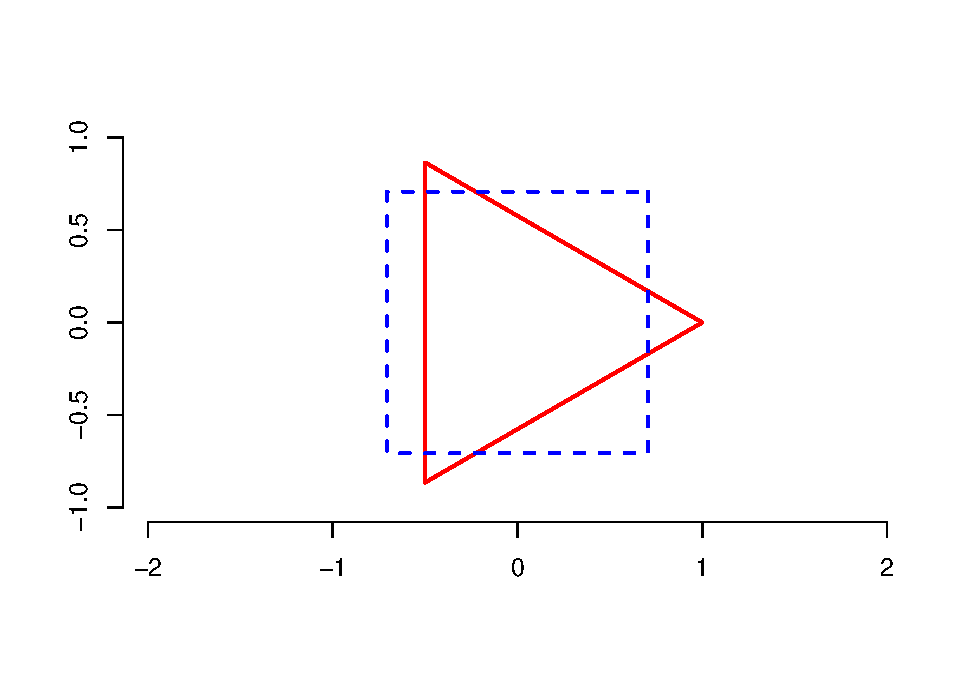
\includegraphics{Assigment4_files/figure-latex/unnamed-chunk-6-1.pdf}

\subsection{2. {[}30 marks{]} Here, we will repeat Question 1 using S4 R
OOP, as
follows.}\label{marks-here-we-will-repeat-question-1-using-s4-r-oop-as-follows.}

\subsubsection{\texorpdfstring{(a) Repeat Question 1(a) but call your
class
``regpolygon4''.}{(a) Repeat Question 1(a) but call your class regpolygon4.}}\label{a-repeat-question-1a-but-call-your-class-regpolygon4.}

\begin{Shaded}
\begin{Highlighting}[]
\KeywordTok{setClass}\NormalTok{(}\StringTok{"regpolygon4"}\NormalTok{,  }
         \KeywordTok{representation}\NormalTok{(}
              \DataTypeTok{x =} \StringTok{"numeric"}\NormalTok{, }
              \DataTypeTok{y =} \StringTok{"numeric"}\NormalTok{, }
              \DataTypeTok{name =} \StringTok{"character"}\NormalTok{, }
              \DataTypeTok{radius =} \StringTok{"numeric"}\NormalTok{,}
              \DataTypeTok{shift =} \StringTok{"numeric"}\NormalTok{,}
              \DataTypeTok{sides =} \StringTok{"numeric"}
\NormalTok{           )}
\NormalTok{         )}

\KeywordTok{setClass}\NormalTok{(}\StringTok{"newregpolygon4"}\NormalTok{, }
         \KeywordTok{representation}\NormalTok{(}
             \DataTypeTok{sides =} \StringTok{"numeric"}
\NormalTok{           ),}
         \DataTypeTok{contains =} \StringTok{"regpolygon4"}
\NormalTok{         )}



\NormalTok{newregpolygon4 <-}\StringTok{ }\ControlFlowTok{function}\NormalTok{(}\DataTypeTok{sides =} \DecValTok{3}\NormalTok{)\{}
  \ControlFlowTok{if}\NormalTok{ (sides }\OperatorTok{<}\StringTok{ }\DecValTok{2}\NormalTok{) \{}
    \KeywordTok{stop}\NormalTok{(}\StringTok{"sides should be greater than or equal to 3"}\NormalTok{)}
\NormalTok{  \} }\ControlFlowTok{else} \ControlFlowTok{if}\NormalTok{ (}\KeywordTok{is.infinite}\NormalTok{(sides)) \{}
\NormalTok{    sides <-}\StringTok{ }\DecValTok{99}
\NormalTok{  \} }\ControlFlowTok{else} \ControlFlowTok{if}\NormalTok{ (sides}\OperatorTok\DecValTok{1} \OperatorTok{!=}\StringTok{ }\DecValTok{0}\NormalTok{) \{}
    \KeywordTok{stop}\NormalTok{(}\StringTok{"sides should be integer"}\NormalTok{)}
\NormalTok{  \}}

  \KeywordTok{regpolygon4}\NormalTok{(}\DataTypeTok{sides =}\NormalTok{ sides, }\DataTypeTok{radius =} \DecValTok{1}\NormalTok{, }\DataTypeTok{shift =} \DecValTok{0}\NormalTok{)}
  
\NormalTok{\}}

\NormalTok{regpolygon4 <-}\StringTok{ }\ControlFlowTok{function}\NormalTok{(sides, radius, shift) \{}
  
\NormalTok{  theta0 <-}\StringTok{ }\NormalTok{shift }\OperatorTok{+}\StringTok{ }\KeywordTok{seq}\NormalTok{(}\DecValTok{0}\NormalTok{, }\DecValTok{2} \OperatorTok{*}\StringTok{ }\NormalTok{pi, }\DataTypeTok{length =}\NormalTok{ sides }\OperatorTok{+}\StringTok{ }\DecValTok{1}\NormalTok{)}
  
  \ControlFlowTok{if}\NormalTok{(sides }\OperatorTok{==}\StringTok{ }\DecValTok{99}\NormalTok{) \{}
\NormalTok{    name <-}\StringTok{ "circle"}
\NormalTok{  \} }\ControlFlowTok{else} \ControlFlowTok{if}\NormalTok{ (sides }\OperatorTok{<}\StringTok{ }\DecValTok{20}\NormalTok{) \{}
\NormalTok{    name <-}\StringTok{ }\ControlFlowTok{switch}\NormalTok{(sides }\OperatorTok{-}\StringTok{ }\DecValTok{2}\NormalTok{, }\StringTok{"triangle"}\NormalTok{, }\StringTok{"square"}\NormalTok{, }\StringTok{"pentagon"}\NormalTok{, }\StringTok{"hexagon"}\NormalTok{, }\StringTok{"heptagon"}\NormalTok{, }\StringTok{"octagon"}\NormalTok{, }\StringTok{"enneagon"}\NormalTok{, }\StringTok{"decagon"}\NormalTok{, }\StringTok{"hendecagon"}\NormalTok{, }\StringTok{"dodecagon"}\NormalTok{, }\StringTok{"triskaidecagon"}\NormalTok{, }\StringTok{"tetrakaidecagon"}\NormalTok{, }\StringTok{"pentakaidecagon"}\NormalTok{, }\StringTok{"hexakaidecagon"}\NormalTok{, }\StringTok{"heptakaidecagon"}\NormalTok{, }\StringTok{"octakaidecagon"}\NormalTok{, }\StringTok{"enneakaidecagon"}\NormalTok{, }\StringTok{"enneakaidecagon"}\NormalTok{)}
\NormalTok{  \} }\ControlFlowTok{else}\NormalTok{ \{}
\NormalTok{    name <-}\StringTok{ }\KeywordTok{paste}\NormalTok{(sides, }\StringTok{"gon"}\NormalTok{, }\DataTypeTok{sep =} \StringTok{"-"}\NormalTok{)}
\NormalTok{  \}}
  
  \KeywordTok{new}\NormalTok{(}\StringTok{"regpolygon4"}\NormalTok{,}
      \DataTypeTok{x =}\NormalTok{ radius }\OperatorTok{*}\StringTok{ }\KeywordTok{round}\NormalTok{(}\KeywordTok{sin}\NormalTok{(theta0), }\DecValTok{4}\NormalTok{), }
      \DataTypeTok{y =}\NormalTok{ radius }\OperatorTok{*}\StringTok{ }\KeywordTok{round}\NormalTok{(}\KeywordTok{cos}\NormalTok{(theta0), }\DecValTok{4}\NormalTok{),}
      \DataTypeTok{name =}\NormalTok{ name,}
      \DataTypeTok{sides =}\NormalTok{ sides,}
      \DataTypeTok{radius =}\NormalTok{ radius,}
      \DataTypeTok{shift =}\NormalTok{ shift}
\NormalTok{  )}
\NormalTok{\}}

\NormalTok{rpg13 <-}\StringTok{ }\KeywordTok{newregpolygon4}\NormalTok{()}
\NormalTok{rpg14 <-}\StringTok{ }\KeywordTok{newregpolygon4}\NormalTok{(}\DataTypeTok{sides =} \DecValTok{4}\NormalTok{) }\CommentTok{# Square}
\NormalTok{rpg18 <-}\StringTok{ }\KeywordTok{newregpolygon4}\NormalTok{(}\DataTypeTok{sides =} \DecValTok{8}\NormalTok{) }\CommentTok{# Octagon}
\NormalTok{rpg1Inf <-}\StringTok{ }\KeywordTok{newregpolygon4}\NormalTok{(}\DataTypeTok{sides =} \OtherTok{Inf}\NormalTok{) }\CommentTok{# Circle}
\end{Highlighting}
\end{Shaded}

\subsubsection{(b) Repeat Question 1(b).}\label{b-repeat-question-1b.}

\begin{Shaded}
\begin{Highlighting}[]
\NormalTok{sides <-}\StringTok{ }\ControlFlowTok{function}\NormalTok{(obj) obj}\OperatorTok{@}\NormalTok{sides}

\NormalTok{radius <-}\StringTok{ }\ControlFlowTok{function}\NormalTok{(obj) \{}
\NormalTok{  firstVertixX <-}\StringTok{ }\NormalTok{obj}\OperatorTok{@}\NormalTok{x[}\DecValTok{1}\NormalTok{]}
\NormalTok{  firstVertixY <-}\StringTok{ }\NormalTok{obj}\OperatorTok{@}\NormalTok{y[}\DecValTok{1}\NormalTok{]}
  
  \KeywordTok{sqrt}\NormalTok{(firstVertixX}\OperatorTok{^}\DecValTok{2} \OperatorTok{+}\StringTok{ }\NormalTok{firstVertixY}\OperatorTok{^}\DecValTok{2}\NormalTok{)}
\NormalTok{\}}

\NormalTok{vertices <-}\StringTok{ }\ControlFlowTok{function}\NormalTok{(obj) \{}
  \KeywordTok{cbind}\NormalTok{(}\DataTypeTok{x =}\NormalTok{ obj}\OperatorTok{@}\NormalTok{x, }\DataTypeTok{y =}\NormalTok{ obj}\OperatorTok{@}\NormalTok{y)}
\NormalTok{\}}

\KeywordTok{radius}\NormalTok{(rpg18)}
\end{Highlighting}
\end{Shaded}

\begin{verbatim}
## [1] 1
\end{verbatim}

\begin{Shaded}
\begin{Highlighting}[]
\KeywordTok{sides}\NormalTok{(rpg18)}
\end{Highlighting}
\end{Shaded}

\begin{verbatim}
## [1] 8
\end{verbatim}

\begin{Shaded}
\begin{Highlighting}[]
\KeywordTok{vertices}\NormalTok{(rpg18)}
\end{Highlighting}
\end{Shaded}

\begin{verbatim}
##             x       y
##  [1,]  0.0000  1.0000
##  [2,]  0.7071  0.7071
##  [3,]  1.0000  0.0000
##  [4,]  0.7071 -0.7071
##  [5,]  0.0000 -1.0000
##  [6,] -0.7071 -0.7071
##  [7,] -1.0000  0.0000
##  [8,] -0.7071  0.7071
##  [9,]  0.0000  1.0000
\end{verbatim}

\subsubsection{(c) Repeat Question 1(c).}\label{c-repeat-question-1c.}

\begin{Shaded}
\begin{Highlighting}[]
\NormalTok{xcoords <-}\StringTok{ }\ControlFlowTok{function}\NormalTok{(obj) obj}\OperatorTok{@}\NormalTok{x}
\NormalTok{ycoords <-}\StringTok{ }\ControlFlowTok{function}\NormalTok{(obj) obj}\OperatorTok{@}\NormalTok{y}
\NormalTok{rcoords <-}\StringTok{ }\ControlFlowTok{function}\NormalTok{(obj) obj}\OperatorTok{@}\NormalTok{radius}
\NormalTok{scoords <-}\StringTok{ }\ControlFlowTok{function}\NormalTok{(obj) obj}\OperatorTok{@}\NormalTok{shift}
\NormalTok{namepoly <-}\StringTok{ }\ControlFlowTok{function}\NormalTok{(obj) obj}\OperatorTok{@}\NormalTok{name}

\KeywordTok{setMethod}\NormalTok{(show, }\KeywordTok{signature}\NormalTok{(}\DataTypeTok{object =} \StringTok{"regpolygon4"}\NormalTok{), }\ControlFlowTok{function}\NormalTok{(object) \{}
  \KeywordTok{print}\NormalTok{(}\StringTok{"This is S3 Object for creating polygons"}\NormalTok{, }\DataTypeTok{quote =} \OtherTok{FALSE}\NormalTok{)}
  \KeywordTok{print}\NormalTok{(}\KeywordTok{paste}\NormalTok{(}\StringTok{"sides "}\NormalTok{, }\KeywordTok{sides}\NormalTok{(object)), }\DataTypeTok{quote =} \OtherTok{FALSE}\NormalTok{)}
  
  \KeywordTok{print}\NormalTok{(}\KeywordTok{paste}\NormalTok{(}\StringTok{"vertex"}\NormalTok{,}\StringTok{"("}\NormalTok{, }
              \KeywordTok{format}\NormalTok{(}\KeywordTok{xcoords}\NormalTok{(object)), }\StringTok{", "}\NormalTok{, }
              \KeywordTok{format}\NormalTok{(}\KeywordTok{ycoords}\NormalTok{(object)), }\StringTok{")"}\NormalTok{, }\DataTypeTok{sep =} \StringTok{""}\NormalTok{), }
        \DataTypeTok{quote =} \OtherTok{FALSE}\NormalTok{)}
  \KeywordTok{print}\NormalTok{(}\KeywordTok{paste}\NormalTok{(}\StringTok{"name "}\NormalTok{, }\KeywordTok{namepoly}\NormalTok{(object)), }\DataTypeTok{quote =} \OtherTok{FALSE}\NormalTok{)}
\NormalTok{\})}

\NormalTok{rpg13}
\end{Highlighting}
\end{Shaded}

\begin{verbatim}
## [1] This is S3 Object for creating polygons
## [1] sides  3
## [1] vertex( 0.000,  1.0) vertex( 0.866, -0.5) vertex(-0.866, -0.5)
## [4] vertex( 0.000,  1.0)
## [1] name  triangle
\end{verbatim}

\begin{Shaded}
\begin{Highlighting}[]
\NormalTok{rpg14}
\end{Highlighting}
\end{Shaded}

\begin{verbatim}
## [1] This is S3 Object for creating polygons
## [1] sides  4
## [1] vertex( 0,  1) vertex( 1,  0) vertex( 0, -1) vertex(-1,  0)
## [5] vertex( 0,  1)
## [1] name  square
\end{verbatim}

\begin{Shaded}
\begin{Highlighting}[]
\NormalTok{rpg18}
\end{Highlighting}
\end{Shaded}

\begin{verbatim}
## [1] This is S3 Object for creating polygons
## [1] sides  8
## [1] vertex( 0.0000,  1.0000) vertex( 0.7071,  0.7071)
## [3] vertex( 1.0000,  0.0000) vertex( 0.7071, -0.7071)
## [5] vertex( 0.0000, -1.0000) vertex(-0.7071, -0.7071)
## [7] vertex(-1.0000,  0.0000) vertex(-0.7071,  0.7071)
## [9] vertex( 0.0000,  1.0000)
## [1] name  octagon
\end{verbatim}

\begin{Shaded}
\begin{Highlighting}[]
\KeywordTok{print}\NormalTok{(rpg18)}
\end{Highlighting}
\end{Shaded}

\begin{verbatim}
## [1] This is S3 Object for creating polygons
## [1] sides  8
## [1] vertex( 0.0000,  1.0000) vertex( 0.7071,  0.7071)
## [3] vertex( 1.0000,  0.0000) vertex( 0.7071, -0.7071)
## [5] vertex( 0.0000, -1.0000) vertex(-0.7071, -0.7071)
## [7] vertex(-1.0000,  0.0000) vertex(-0.7071,  0.7071)
## [9] vertex( 0.0000,  1.0000)
## [1] name  octagon
\end{verbatim}

\subsubsection{(d) Repeat Question 1(d)}\label{d-repeat-question-1d}

\begin{Shaded}
\begin{Highlighting}[]
\KeywordTok{setMethod}\NormalTok{(}\StringTok{"plot"}\NormalTok{, }\KeywordTok{c}\NormalTok{(}\StringTok{"regpolygon4"}\NormalTok{), }\ControlFlowTok{function}\NormalTok{(x, }\DataTypeTok{y=}\OtherTok{NULL}\NormalTok{, }\DataTypeTok{z=}\OtherTok{NULL}\NormalTok{, ...) \{}
  
  \KeywordTok{plot.new}\NormalTok{()}
  \KeywordTok{plot.window}\NormalTok{(}\DataTypeTok{xlim =} \KeywordTok{c}\NormalTok{(}\OperatorTok{-}\DecValTok{1}\NormalTok{, }\DecValTok{1}\NormalTok{), }\DataTypeTok{ylim =} \KeywordTok{c}\NormalTok{(}\OperatorTok{-}\DecValTok{1}\NormalTok{, }\DecValTok{1}\NormalTok{), }\DataTypeTok{asp =} \DecValTok{1}\NormalTok{)}
  \KeywordTok{axis}\NormalTok{(}\DecValTok{1}\NormalTok{)}
  \KeywordTok{axis}\NormalTok{(}\DecValTok{2}\NormalTok{)}
  
\NormalTok{  object <-}\StringTok{ }\KeywordTok{c}\NormalTok{(x, y, z)}
\NormalTok{  params <-}\StringTok{ }\KeywordTok{list}\NormalTok{(...)}
  
  \CommentTok{#Detecting further objects of regpolygon3 in optional parametes}
  \ControlFlowTok{for}\NormalTok{(i }\ControlFlowTok{in} \DecValTok{1}\OperatorTok{:}\KeywordTok{length}\NormalTok{(params)) \{}
    \ControlFlowTok{if}\NormalTok{(}\KeywordTok{inherits}\NormalTok{(}\KeywordTok{...elt}\NormalTok{(i), }\StringTok{"regpolygon4"}\NormalTok{)) \{}
\NormalTok{      object <-}\StringTok{ }\KeywordTok{c}\NormalTok{(object, }\KeywordTok{...elt}\NormalTok{(i))}
\NormalTok{    \}}
\NormalTok{  \}}
  
  \CommentTok{# detected object lengths}
\NormalTok{  len <-}\StringTok{ }\KeywordTok{length}\NormalTok{(object)}
  \ControlFlowTok{if}\NormalTok{(len }\OperatorTok{>}\StringTok{ }\DecValTok{3}\NormalTok{)}
\NormalTok{    params <-}\StringTok{ }\NormalTok{params[}\KeywordTok{names}\NormalTok{(params)][(len}\OperatorTok{-}\DecValTok{2}\NormalTok{)}\OperatorTok{:}\KeywordTok{length}\NormalTok{(params)]}
  
  \ControlFlowTok{if}\NormalTok{(}\KeywordTok{length}\NormalTok{(params[[}\StringTok{"lty"}\NormalTok{]]) }\OperatorTok{>}\StringTok{ }\DecValTok{0} \OperatorTok{&&}\StringTok{ }\KeywordTok{length}\NormalTok{(params[[}\StringTok{"lty"}\NormalTok{]]) }\OperatorTok{<}\StringTok{ }\NormalTok{len) \{}
\NormalTok{    params[[}\StringTok{"lty"}\NormalTok{]] <-}\StringTok{ }\KeywordTok{rep}\NormalTok{(params[[}\StringTok{"lty"}\NormalTok{]], len)}
\NormalTok{  \}}
  
  \ControlFlowTok{if}\NormalTok{(}\KeywordTok{length}\NormalTok{(params[[}\StringTok{"lwd"}\NormalTok{]]) }\OperatorTok{>}\StringTok{ }\DecValTok{0} \OperatorTok{&&}\StringTok{ }\KeywordTok{length}\NormalTok{(params[[}\StringTok{"lwd"}\NormalTok{]]) }\OperatorTok{<}\StringTok{ }\NormalTok{len) \{}
\NormalTok{    params[[}\StringTok{"lwd"}\NormalTok{]] <-}\StringTok{ }\KeywordTok{rep}\NormalTok{(params[[}\StringTok{"lwd"}\NormalTok{]], len)}
\NormalTok{  \}}
  
  \ControlFlowTok{if}\NormalTok{(}\KeywordTok{length}\NormalTok{(params[[}\StringTok{"border"}\NormalTok{]]) }\OperatorTok{>}\StringTok{ }\DecValTok{0} \OperatorTok{&&}\StringTok{ }\KeywordTok{length}\NormalTok{(params[[}\StringTok{"border"}\NormalTok{]]) }\OperatorTok{<}\StringTok{ }\NormalTok{len) \{}
\NormalTok{    params[[}\StringTok{"border"}\NormalTok{]] <-}\StringTok{ }\KeywordTok{rep}\NormalTok{(params[[}\StringTok{"border"}\NormalTok{]], len)}
\NormalTok{  \}}
  
\NormalTok{  r <-}\StringTok{ }\DecValTok{1}
  \ControlFlowTok{for}\NormalTok{(i }\ControlFlowTok{in} \DecValTok{1}\OperatorTok{:}\NormalTok{len) \{}
    
\NormalTok{    x <-}\StringTok{ }\NormalTok{object[[i]]}\OperatorTok{@}\NormalTok{x}
\NormalTok{    y <-}\StringTok{ }\NormalTok{object[[i]]}\OperatorTok{@}\NormalTok{y}
    
    \ControlFlowTok{if}\NormalTok{(object[[i]]}\OperatorTok{@}\NormalTok{radius }\OperatorTok{>}\StringTok{ }\NormalTok{r) \{}
\NormalTok{      r <-}\StringTok{ }\NormalTok{object[[i]]}\OperatorTok{@}\NormalTok{radius}
      \KeywordTok{plot.window}\NormalTok{(}\DataTypeTok{xlim =} \KeywordTok{c}\NormalTok{(}\OperatorTok{-}\NormalTok{r, r), }\DataTypeTok{ylim =} \KeywordTok{c}\NormalTok{(}\OperatorTok{-}\NormalTok{r, r), }\DataTypeTok{asp =} \DecValTok{1}\NormalTok{)}
\NormalTok{    \}}
    
\NormalTok{    border <-}\StringTok{ }\KeywordTok{ifelse}\NormalTok{(}\KeywordTok{any}\NormalTok{(}\KeywordTok{names}\NormalTok{(params) }\OperatorTok{==}\StringTok{ "border"}\NormalTok{), params[[}\StringTok{"border"}\NormalTok{]][i], }\DecValTok{1}\NormalTok{)}
\NormalTok{    lty <-}\StringTok{ }\KeywordTok{ifelse}\NormalTok{(}\KeywordTok{any}\NormalTok{(}\KeywordTok{names}\NormalTok{(params) }\OperatorTok{==}\StringTok{ "lty"}\NormalTok{), params[[}\StringTok{"lty"}\NormalTok{]][i], }\DecValTok{1}\NormalTok{)}
\NormalTok{    lwd <-}\StringTok{ }\KeywordTok{ifelse}\NormalTok{(}\KeywordTok{any}\NormalTok{(}\KeywordTok{names}\NormalTok{(params) }\OperatorTok{==}\StringTok{ "lwd"}\NormalTok{), params[[}\StringTok{"lwd"}\NormalTok{]][i], }\DecValTok{1}\NormalTok{)}
\NormalTok{    col <-}\StringTok{ }\KeywordTok{ifelse}\NormalTok{(}\KeywordTok{any}\NormalTok{(}\KeywordTok{names}\NormalTok{(params) }\OperatorTok{==}\StringTok{ "col"}\NormalTok{), params[[}\StringTok{"col"}\NormalTok{]][i], }\OtherTok{NA}\NormalTok{)}
    
    \KeywordTok{polygon}\NormalTok{(}\DataTypeTok{x =}\NormalTok{ x, }\DataTypeTok{y =}\NormalTok{ y, }\DataTypeTok{border =}\NormalTok{ border, }\DataTypeTok{lty =}\NormalTok{ lty, }\DataTypeTok{lwd =}\NormalTok{ lwd)}
\NormalTok{  \}}
  
\NormalTok{\})}

\KeywordTok{plot}\NormalTok{(rpg13, rpg14, rpg18, }\DataTypeTok{border =} \DecValTok{1}\OperatorTok{:}\DecValTok{3}\NormalTok{, }\DataTypeTok{lty =} \DecValTok{1}\OperatorTok{:}\DecValTok{3}\NormalTok{, }\DataTypeTok{lwd =} \KeywordTok{c}\NormalTok{(}\DecValTok{2}\NormalTok{, }\DecValTok{2}\NormalTok{, }\DecValTok{3}\NormalTok{))}
\end{Highlighting}
\end{Shaded}

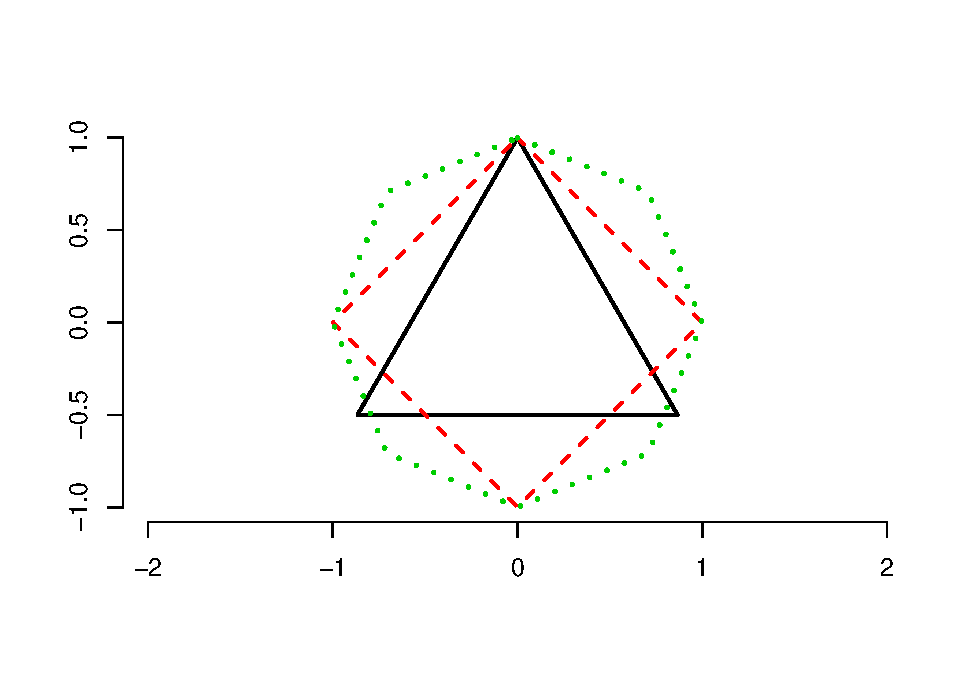
\includegraphics{Assigment4_files/figure-latex/unnamed-chunk-10-1.pdf}

\subsubsection{(e) Repeat Question 1(e).}\label{e-repeat-question-1e.}

\paragraph{(i)}\label{i}

\begin{Shaded}
\begin{Highlighting}[]
\KeywordTok{setMethod}\NormalTok{(}\StringTok{"+"}\NormalTok{, }\KeywordTok{signature}\NormalTok{(}\DataTypeTok{e1 =} \StringTok{"numeric"}\NormalTok{, }\DataTypeTok{e2 =} \StringTok{"regpolygon4"}\NormalTok{), }\ControlFlowTok{function}\NormalTok{(e1, e2) \{ }
  \ControlFlowTok{if}\NormalTok{ (}\KeywordTok{length}\NormalTok{(e1) }\OperatorTok{!=}\StringTok{ }\DecValTok{1} \OperatorTok{&&}\StringTok{ }\OperatorTok{!}\KeywordTok{is.numeric}\NormalTok{(e1)) }
      \KeywordTok{stop}\NormalTok{(}\StringTok{"First parameter should be a number"}\NormalTok{) }
\NormalTok{    sides <-}\StringTok{ }\KeywordTok{sides}\NormalTok{(e2)}
\NormalTok{    r <-}\StringTok{ }\KeywordTok{rcoords}\NormalTok{(e2)}
\NormalTok{    s <-}\StringTok{ }\KeywordTok{scoords}\NormalTok{(e2)}
\NormalTok{    a <-}\StringTok{ }\NormalTok{e1 }
  \KeywordTok{regpolygon4}\NormalTok{(sides, r, a) }
\NormalTok{\})}

\KeywordTok{setMethod}\NormalTok{(}\StringTok{"+"}\NormalTok{, }\KeywordTok{signature}\NormalTok{(}\DataTypeTok{e1 =} \StringTok{"regpolygon4"}\NormalTok{, }\DataTypeTok{e2 =} \StringTok{"numeric"}\NormalTok{), }\ControlFlowTok{function}\NormalTok{(e1, e2) \{ }
  \ControlFlowTok{if}\NormalTok{ (}\KeywordTok{length}\NormalTok{(e2) }\OperatorTok{!=}\StringTok{ }\DecValTok{1} \OperatorTok{&&}\StringTok{ }\OperatorTok{!}\KeywordTok{is.numeric}\NormalTok{(e2)) }
      \KeywordTok{stop}\NormalTok{(}\StringTok{"Second parameter should be a number"}\NormalTok{) }
\NormalTok{    sides <-}\StringTok{ }\KeywordTok{sides}\NormalTok{(e1)}
\NormalTok{    r <-}\StringTok{ }\KeywordTok{rcoords}\NormalTok{(e1)}
\NormalTok{    s <-}\StringTok{ }\KeywordTok{scoords}\NormalTok{(e1)}
\NormalTok{    a <-}\StringTok{ }\NormalTok{e2 }
  \KeywordTok{regpolygon4}\NormalTok{(sides, r, a) }
\NormalTok{\})}

\KeywordTok{setMethod}\NormalTok{(}\StringTok{"*"}\NormalTok{, }\KeywordTok{signature}\NormalTok{(}\DataTypeTok{e1 =} \StringTok{"numeric"}\NormalTok{, }\DataTypeTok{e2 =} \StringTok{"regpolygon4"}\NormalTok{), }\ControlFlowTok{function}\NormalTok{(e1, e2) \{ }
  \ControlFlowTok{if}\NormalTok{ (}\KeywordTok{length}\NormalTok{(e1) }\OperatorTok{!=}\StringTok{ }\DecValTok{1} \OperatorTok{&&}\StringTok{ }\OperatorTok{!}\KeywordTok{is.numeric}\NormalTok{(e1)) }
      \KeywordTok{stop}\NormalTok{(}\StringTok{"First parameter should be a number"}\NormalTok{) }
\NormalTok{    sides <-}\StringTok{ }\KeywordTok{sides}\NormalTok{(e2)}
\NormalTok{    r <-}\StringTok{ }\KeywordTok{rcoords}\NormalTok{(e2)}
\NormalTok{    s <-}\StringTok{ }\KeywordTok{scoords}\NormalTok{(e2)}
\NormalTok{    a <-}\StringTok{ }\NormalTok{e1 }
  \KeywordTok{regpolygon4}\NormalTok{(sides, a, s) }
\NormalTok{\})}

\KeywordTok{setMethod}\NormalTok{(}\StringTok{"*"}\NormalTok{, }\KeywordTok{signature}\NormalTok{(}\DataTypeTok{e1 =} \StringTok{"regpolygon4"}\NormalTok{, }\DataTypeTok{e2 =} \StringTok{"numeric"}\NormalTok{), }\ControlFlowTok{function}\NormalTok{(e1, e2) \{ }
  \ControlFlowTok{if}\NormalTok{ (}\KeywordTok{length}\NormalTok{(e2) }\OperatorTok{!=}\StringTok{ }\DecValTok{1} \OperatorTok{&&}\StringTok{ }\OperatorTok{!}\KeywordTok{is.numeric}\NormalTok{(e2)) }
      \KeywordTok{stop}\NormalTok{(}\StringTok{"Second parameter should be a number"}\NormalTok{) }
\NormalTok{    sides <-}\StringTok{ }\KeywordTok{sides}\NormalTok{(e1)}
\NormalTok{    r <-}\StringTok{ }\KeywordTok{rcoords}\NormalTok{(e1)}
\NormalTok{    s <-}\StringTok{ }\KeywordTok{scoords}\NormalTok{(e1)}
\NormalTok{    a <-}\StringTok{ }\NormalTok{e2 }
  \KeywordTok{regpolygon4}\NormalTok{(sides, a, s) }
\NormalTok{\})}


\NormalTok{## Sample Results}
\FloatTok{0.5} \OperatorTok{+}\StringTok{ }\NormalTok{rpg13}
\end{Highlighting}
\end{Shaded}

\begin{verbatim}
## [1] This is S3 Object for creating polygons
## [1] sides  3
## [1] vertex( 0.4794,  0.8776) vertex( 0.5203, -0.8540)
## [3] vertex(-0.9997, -0.0236) vertex( 0.4794,  0.8776)
## [1] name  triangle
\end{verbatim}

\begin{Shaded}
\begin{Highlighting}[]
\NormalTok{rpg13 }\OperatorTok{*}\StringTok{ }\DecValTok{3}
\end{Highlighting}
\end{Shaded}

\begin{verbatim}
## [1] This is S3 Object for creating polygons
## [1] sides  3
## [1] vertex( 0.000,  3.0) vertex( 2.598, -1.5) vertex(-2.598, -1.5)
## [4] vertex( 0.000,  3.0)
## [1] name  triangle
\end{verbatim}

\begin{Shaded}
\begin{Highlighting}[]
\NormalTok{## Verification Results}
\FloatTok{0.5} \OperatorTok{+}\StringTok{ }\DecValTok{3} \OperatorTok{*}\StringTok{ }\NormalTok{rpg13}
\end{Highlighting}
\end{Shaded}

\begin{verbatim}
## [1] This is S3 Object for creating polygons
## [1] sides  3
## [1] vertex( 1.4382,  2.6328) vertex( 1.5609, -2.5620)
## [3] vertex(-2.9991, -0.0708) vertex( 1.4382,  2.6328)
## [1] name  triangle
\end{verbatim}

\begin{Shaded}
\begin{Highlighting}[]
\DecValTok{3} \OperatorTok{*}\StringTok{ }\NormalTok{(}\FloatTok{0.5} \OperatorTok{+}\StringTok{ }\NormalTok{rpg13)}
\end{Highlighting}
\end{Shaded}

\begin{verbatim}
## [1] This is S3 Object for creating polygons
## [1] sides  3
## [1] vertex( 1.4382,  2.6328) vertex( 1.5609, -2.5620)
## [3] vertex(-2.9991, -0.0708) vertex( 1.4382,  2.6328)
## [1] name  triangle
\end{verbatim}

\paragraph{(ii)}\label{ii}

\begin{Shaded}
\begin{Highlighting}[]
\KeywordTok{plot}\NormalTok{(rpg13 }\OperatorTok{+}\StringTok{ }\NormalTok{pi}\OperatorTok{/}\DecValTok{2}\NormalTok{, }\DecValTok{2} \OperatorTok{*}\StringTok{ }\NormalTok{rpg14 }\OperatorTok{+}\StringTok{ }\NormalTok{pi}\OperatorTok{/}\DecValTok{4}\NormalTok{, }\DataTypeTok{border =} \KeywordTok{c}\NormalTok{(}\DecValTok{2}\NormalTok{, }\DecValTok{4}\NormalTok{), }\DataTypeTok{lty =} \DecValTok{1}\OperatorTok{:}\DecValTok{2}\NormalTok{, }\DataTypeTok{lwd =} \DecValTok{2}\NormalTok{)}
\end{Highlighting}
\end{Shaded}

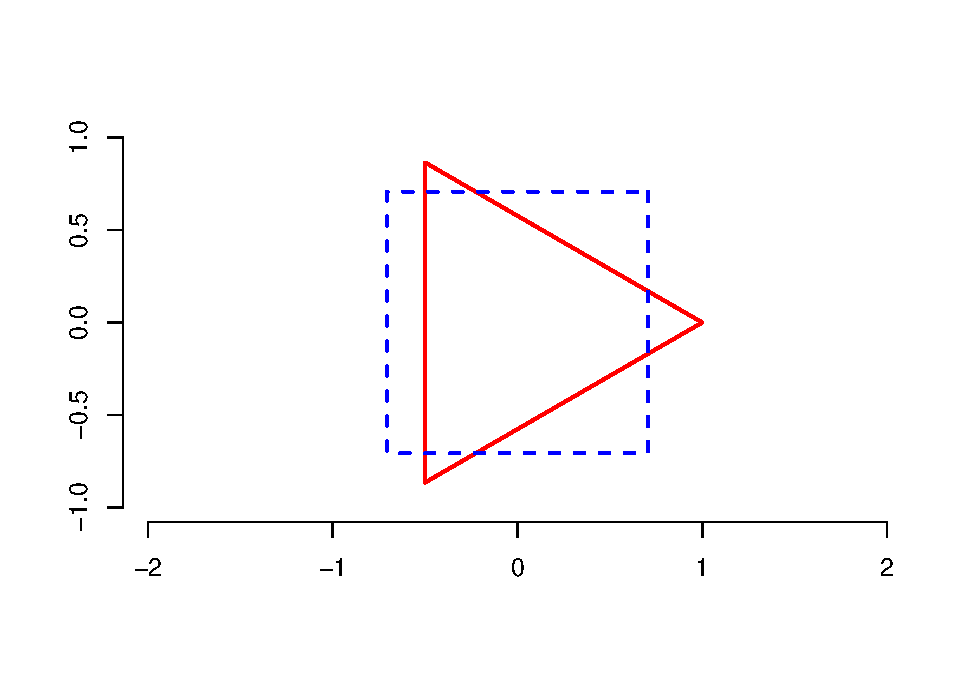
\includegraphics{Assigment4_files/figure-latex/unnamed-chunk-12-1.pdf}


\end{document}
